% -*-coding: utf-8 -*-
% Держать в начале каждого файла!

\documentclass[a4paper, 12pt]{extarticle}
% 14 пт - жесть
\usepackage{metod}

\MTDSetPhysSection{Механика}
\MTDSetTitle{Условия равновесия твердого тела с~закрепленной осью вращения}
\MTDDesignator{М--6}
\MTDSetGrade{10}

\MTDSetAuthors{И.~Н.~Грачева, В.~И.~Гребенкин, А.~Е.~Иванов, И.~А.~Коротова,
Е.~И.~Красавина, А.~В.~Кравцов, Н.~С.~Кулеба, Б.~В.~Падалкин,
Г.~Ю.~Шевцова, Т.~С.~Цвецинская}

\MTDSetEditorsGenCase{И.~Н.~Грачевой, А.~Е.~Иванова, А.~В.~Кравцова}

\newcommand{\eps}{\epsilon}
\newcommand{\nisum}{\sum\limits_{i=1}^{i=n}} %WTF?!
\newcommand{\isum}{\sum\limits_{i=1}^{n}}
\newcommand{\issum}{\sum\limits_{i}}

\begin{document}
\MTDTitlePage
\MTDInfoPage

\setcounter{section}{6}

\subsection{Цель работы}
Целью работы является экспериментальная проверка условий равновесия тела с закрепленной осью вращения.

\subsection{Основные теоретические сведения}
Твердое тело с закрепленной неподвижной осью вращения остается в  покое, если сумма моментов сил, действующих на тело, относительно оси вращения равна нулю:
\begin{equation}
\label{eq:m6-moment}
\isum M_i = 0. % Точку поставил
\end{equation}

При этом сумма сил, действующих на тело, также равна нулю из-за возникновения сил реакций со стороны крепления оси вращения.

\subsection{Описание экспериментальной установки}

\begin{figure}[h]
\begin{center}
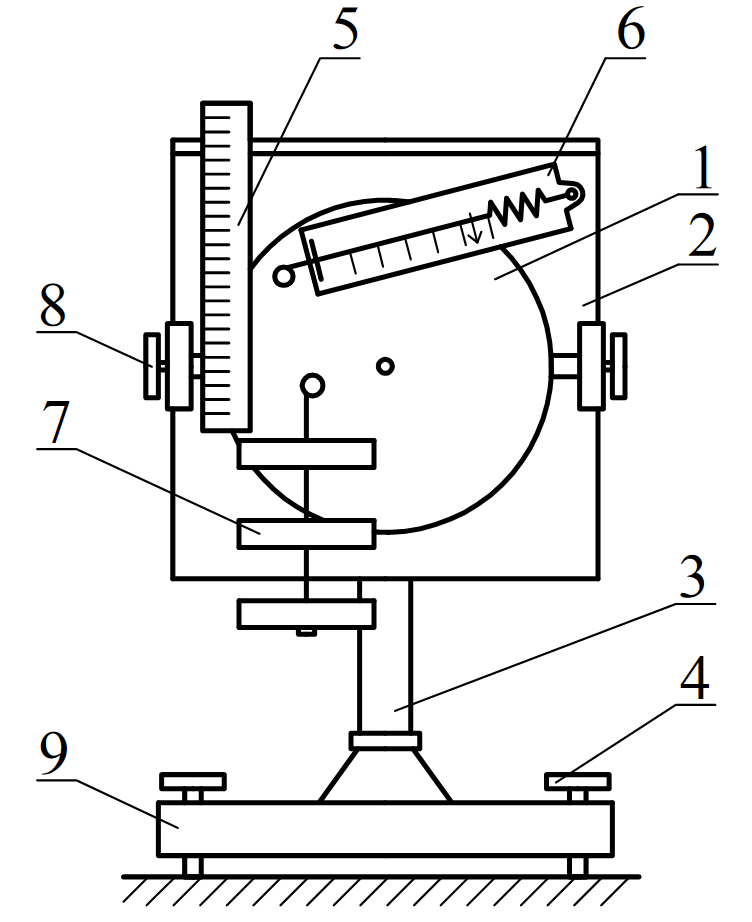
\includegraphics[width=0.35\linewidth, keepaspectratio=true]{M6-MechEquilibriumMachine}
\end{center}
\caption{Схема установки \label{fig:m6-disk-device}}
\end{figure}

Установка изображена на рис.~\ref{fig:m6-disk-device}. В установке неоднородный диск~\emph{1} может поворачиваться вокруг горизонтальной оси, проходящей через его геометрический центр. Положение диска с помощью указателя определяется по круговой шкале, деления которой нанесены на раме~\emph{2}, укрепленной на стойке~\emph{3}. Боковыми винтами~\emph{8} фиксируют положение диска.  Установка всего прибора по отвесу производится регулировочными винтами~\emph{4} в плите~\emph{9}. Изменение высоты центра масс фиксируется по шкале вертикальной линейки~\emph{5}. Динамометр~\emph{6} шарнирно прикрепляется одним концом к раме, другим "--- к диску. При повороте диска пружина растягивается. Сила натяжения пружины измеряется по шкале динамометра. К диску на тонкой нити подвешиваются грузы~\emph{7}. Вес диска измеряется спаренным динамометром, не входящим в состав установки и расположенном на столе рядом с описанной  установкой. % не знаю, специально или нет, ты убрал абзацы, мб это правильная мысль

\subsection{Порядок выполнения работы}
\begin{enumerate}
\item Во время домашней подготовки к  работе  выполните в лабораторном журнале таблицы~\ref{tab:m6-first}--\ref{tab:m6-third}.
\item Ознакомьтесь с установкой и получите у преподавателя допуск к выполнению работы.
\end{enumerate}

\begin{table}[h] %поменяла таблицу в соответствии со своей тетрадью и логикой
\caption{\label{tab:m6-first}} %мб растянуть и сделать \multirow везде
\begin{center}
\begin{tabular}{|>{\centering\arraybackslash} m{0.5cm}|>{\centering\arraybackslash} m{0.5cm}|>{\centering\arraybackslash} m{0.5cm}|c|>{\centering\arraybackslash} m{0.5cm}|>{\centering\arraybackslash} m{0.5cm}|>{\centering\arraybackslash} m{0.5cm}|c|}
\hline
\multicolumn{3}{|c|}{$P_i$,~\Units{Н}} & \multirow{2}*{$T$,~\Units{Н}} & \multicolumn{3}{c|}{$F_i$,~\Units{Н}} & \multirow{2}*{$N$,~\Units{Н}} \\ \cline{1-3} \cline{5-7}
1 & 2 & 3 & & 1 & 2 & 3 & \\ \hline
& & & & & & & \\ \hline
\multicolumn{3}{|c|}{\multirow{2}*{$\hspace{3pt}\MTDMean{P} \pm \Delta P$,~\Units{Н}}} &  \multirow{2}*{$T \pm \Delta T$,~\Units{Н}} & \multicolumn{3}{c|}{\multirow{2}*{$\hspace{3pt}\MTDMean{F} \pm \Delta F$,~\Units{Н}}} & \multirow{2}*{$N \pm \Delta N$,~\Units{Н}} \\
\multicolumn{3}{|c|}{} & & \multicolumn{3}{c|}{} & \\ \hline
\multicolumn{3}{|c|}{} & & \multicolumn{3}{c|}{} & \\ \hline
\end{tabular}
\end{center}
\end{table}

\begin{table}[h]
\caption{\label{tab:m6-second}}
\begin{center}
\begin{tabular}{|c|>{\centering\arraybackslash} m{1.35cm}|c|>{\centering\arraybackslash} m{1.35cm}|c|>{\centering\arraybackslash} m{1.35cm}|}
\hline
\multirow{2}*{$d_P \pm \Delta d_P$,~\Units{мм}} & & \multirow{2}*{$d_T \pm \Delta d_T$,~\Units{мм}} & & \multirow{2}*{$d_F \pm \Delta d_F$,~\Units{мм}} & \\
& & & & & \\ \hline
\multirow{2}*{$P \pm \Delta P$,~\Units{Н}} & & \multirow{2}*{$T \pm \Delta T$,~\Units{Н}} & & \multirow{2}*{$F \pm \Delta F$,~\Units{Н}} & \\
& & & & & \\ \hline
\multirow{2}*{$M_P \pm \Delta M_P,~\Units{\text{Н} \cdot \text{м}}$} & & \multirow{2}*{$M_T \pm \Delta M_T,~\Units{\text{Н} \cdot \text{м}}$} & & \multirow{2}*{$M_F \pm \Delta M_F,~\Units{\text{Н} \cdot \text{м}}$} & \\
& & & & & \\ \hline
\end{tabular}
\end{center}
\end{table}

\begin{table}[h]
\caption{\label{tab:m6-third}}
\begin{center}
\begin{tabular}{|c|>{\centering\arraybackslash} m{1.35cm}|c|>{\centering\arraybackslash} m{1.35cm}|c|}
\hline
\multirow{2}*{$d'_P \pm \Delta d'_P$,~\Units{мм}} & & \multirow{2}*{$d'_N \pm \Delta d'_N$,~\Units{мм}} & & \multirow{4}*{$M' \pm \Delta M',~\Units{\text{Н} \cdot \text{м}}$} \\
& & & & \\ \cline{1-4}
\multirow{2}*{$P \pm \Delta P$,~\Units{Н}} & & \multirow{2}*{$N \pm \Delta N$,~\Units{Н}} & &  \\
& & & & \\ \hline
\multirow{2}*{$M'_P \pm \Delta M'_P,~\Units{\text{Н} \cdot \text{м}}$} & & \multirow{2}*{$M'_N \pm \Delta M'_N,~\Units{\text{Н} \cdot \text{м}}$} & & \\
& & & & \\ \hline
\end{tabular}
\end{center}
\end{table}

Расчетные соотношения к таблицам~\ref{tab:m6-second} и \ref{tab:m6-third}: \\
$\Delta d$ "--- приборная погрешность измерительной линейки; \\
значения $P$, $T$, $F$, $\Delta P$, $\Delta T$, $\Delta F$ берутся из таблицы~\ref{tab:m6-first}; \\
\[
\Delta M_P = \sqrt{(d_P \Delta P) ^2 + (P \Delta d_P) ^2};
\]
для $\Delta M_T$ и $\Delta M_F$ "--- аналогично; \\
\begin{equation} %дала этой формуле номер, потому что непонятно чем она отличается от формулы ниже про реакцию опоры
\label{eq:m6-moment-error}
\Delta M = \MTDMean{M} \sqrt{\left( \frac{\Delta M_P}{M_P} \right) ^2 + \left( \frac{\Delta M_T}{M_T} \right) ^2 + \left( \frac{\Delta M_F}{M_F} \right) ^2 }.
\end{equation}


\MTDTask{Определение массы и положения центра тяжести неоднородного диска.}
\begin{enumerate}
\item
С помощью спаренного динамометра, укрепленного на штативе,
взвесьте три раза диск. Измеренные значения силы тяжести~$P_i$ запишите в таблицу~\ref{tab:m6-first}. % ИЗМ Было: Пользуясь разделом В.4 настоящего сборника,
Пользуясь разделом~В.4 вводной лабораторной работы, определите погрешность измерения~$P$.
\item
Найдите положение центра тяжести диска следующим образом.
Прикрепив к диску лист миллиметровой бумаги с вырезом посередине (вырез должен быть сделан так, чтобы пересечение двух взаимно перпендикулярных утолщенных линий <<миллиметровки>> проходило через центр диска), подвесьте диск вместе с отвесом последовательно в трех точках диска. На пересечении трех прямых, проведенных по отвесу, отметьте точкой положение центра тяжести. Если на пересечении прямых образуется маленький треугольник, то точку центра тяжести ставят в точке пересечения медиан этого треугольника.
\end{enumerate}

\MTDTask{Определение силы реакции~$\vec{N}$, действующей на диск со стороны оси вращения.}
\begin{enumerate}
\item Надев диск на ось, прикрепите к нему динамометр и подвесьте на нити грузы такой массы, чтобы пружинка растянулась примерно вдвое. Диск, остановившийся в положении равновесия, закрепите стопорными винтами. Запишите показания~$F$ динамометра в таблицу~\ref{tab:m6-first}. Проведите на миллиметровке линии действия силы упругости~$\vec{F}$ пружины динамометра, силы натяжения~$\vec{T}$ нити крепления грузов и силы тяжести~$\vec{P}$. Сила тяжести приложена к центру тяжести. 
\item Освободив стопорные винты, повторите измерения по п.~1 еще два раза. Результаты запишите в таблицу~\ref{tab:m6-first}.
\item По массам грузов определите силу натяжения~$\vec{T}$ нити. Относительную погрешность определения силы~$\vec{T}$ считать равной 1\%. 
\item Определите силу реакции~$\vec{N}$ графическим способом. На листе миллиметровой бумаги в определенном масштабе отложите векторы $\vec{P} + \vec{T}$, $\vec{F}$ так, как показано на рис.~\ref{fig:m6-scheme}. \\
Используя условие равновесия системы
\begin{equation}
\label{eq:m6-balance}
\vec{F} + \vec{P} + \vec{T} + \vec{N} = 0,
\end{equation}
получаем
\begin{equation}
\label{eq:m6-reaction-force}
-\vec{N} = \vec{F} + \vec{P} + \vec{T}.
\end{equation}

\begin{figure}[h]
\begin{center}
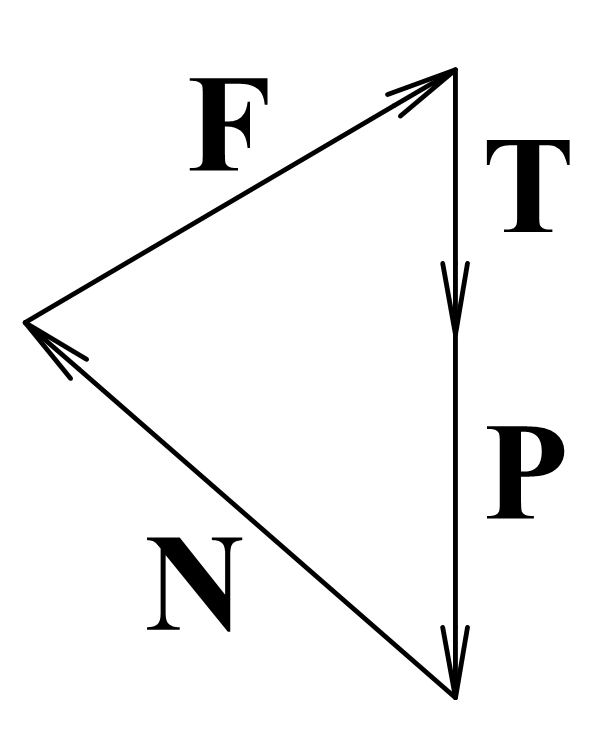
\includegraphics[width=0.15\linewidth, keepaspectratio=true]{M6-ForceTriangle}
\end{center}
\caption{Расчет силы реакции опор \label{fig:m6-scheme}}
\end{figure}

Следовательно, для нахождения вектора~$\vec{N}$ необходимо соединить конец вектора~$\vec{P}$ и начало вектора~$\vec{F}$. Значение модуля $N$ запишите в таблицу~\ref{tab:m6-first}. Рассчитайте погрешность измерения $N$ по выражению
\begin{equation}
\label{eq:m6-reaction-force-error}
\Delta N = \MTDMean{N} \sqrt{\left( \frac{\Delta P}{P} \right) ^2 + \left( \frac{\Delta T}{T} \right) ^2 + \left( \frac{\Delta F}{F} \right) ^2}.
\end{equation}
\end{enumerate}

\MTDTask{Изучение правила моментов.}
\begin{enumerate}
\item Снимите миллиметровую бумагу с диска, с обратной стороны заклейте отверстие бумагой. Обозначьте точкой ось вращения диска. Измерьте плечи~$d_p$, $d_F$, $d_T$ сил~$\vec{P}$, $\vec{T}$, $\vec{F}$ относительно оси вращения диска.
\item Выполнив необходимые расчеты, заполните таблицу~\ref{tab:m6-second}.
\item Убедитесь, что правило моментов справедливо для любой оси, параллельной той, вокруг которой тело вращается в действительности. Рассмотрите ось, перпендикулярную плоскости диска и проходящую через точку пересечения линий действия сил~$\vec{T}$ и $\vec{F}$. Измерьте плечи~$d'_P$ и $d'_N$ сил~$\vec{P}$ и $\vec{N}$ относительно этой оси, запишите результаты в таблицу~\ref{tab:m6-third}. Сопоставив результаты измерений по таблицам~\ref{tab:m6-second} и \ref{tab:m6-third}, сделайте выводы и напишите заключение к работе.
\end{enumerate}

\subsection{Контрольные вопросы}
\begin{enumerate}
\item Сформулируйте условия равновесия твердого тела с закрепленной осью вращения. 
\item Тело находится на закрепленной оси вращения. Как должна проходить  линия действия силы, приложенной к телу, чтобы оно находилось в состоянии равновесия?
\item Может ли тело, находящееся в равновесии, двигаться поступательно или вращаться?
\end{enumerate}


\end{document} 